\section{Implementation-Aligned Projections}\label{proj}

This section replaces the first-order projection model with one that matches
the implemented protocol. The v1 model used a single latency value \(l\) and
treated it as a representative network latency. The implementation requires a
more precise model: a quorum stage can advance once the required
supermajority has arrived, so finality is governed by the slowest member of
the fastest safe supermajority, not by arithmetic average latency.

\subsection{Protocol Throughput and Finality}\label{proj:tps}

We use the following variables:

\begin{description}
\item[\(n\)] active validator count.
\item[\(q\)] quorum size. The current implementation uses \(q=6\).
\item[\(R(n,q)\)] number of deterministic quorum rounds selected by the
implementation.
\item[\(S(x)\)] implemented supermajority threshold, where
\(S(x)=x-\lfloor x/3 \rfloor\).
\item[\(F(x)\)] Byzantine safety bound, where
\(F(x)=\lfloor (x-1)/3 \rfloor\).
\item[\(\beta\)] transactions per block.
\item[\(\tau\)] transaction payload size in bytes.
\item[\(E\)] block utilization, \(0 \le E \le 1\).
\item[\(b_{1/3}\)] bandwidth of the lower-third infrastructure class, measured
in bytes per second.
\item[\(t_{1/3}\)] thread count of the lower-third infrastructure class.
\item[\(\nu_{1/3}\)] signature verifications per second per thread for the
lower-third infrastructure class.
\end{description}

The implemented finality model must also include a latency distribution. Let
\(\delta_{u,v}^{(a)}\) be the one-way latency from sender \(u\) to receiver
\(v\) during stage \(a\). For a quorum \(Q\), define the stage latency ceiling
for receiver \(v\) as the \(S(|Q|)\)-th order statistic of the valid arrivals:
\[
\lambda_{a}(Q,v)
=
\operatorname{os}_{S(|Q|)}
\left(
\left\{
\delta_{u,v}^{(a)} : u \in Q
\right\}
\right).
\]
The local node's own vote may be represented with latency \(0\). With
\(q=6\), the threshold is \(S(6)=4\), so this expression waits for the fourth
valid vote and excludes the two slowest or absent validators from the liveness
ceiling.

The quorum stage latency is the slowest receiver that must participate in the
accepted supermajority:
\[
\Lambda_a(Q)
=
\operatorname{os}_{S(|Q|)}
\left(
\left\{
\lambda_a(Q,v) : v \in Q
\right\}
\right).
\]
This is the boundary between the fastest two-thirds and the slowest one-third
of the quorum. It is intentionally not the mean latency. Average latency can be
reported as an operational diagnostic, but it must not be used as the finality
ceiling for a Byzantine-tolerant model.

Let \(A_m\) be the ordered stage list for mode \(m\). For the trusted path,
\[
A_{\mathrm{trusted}}=\{\mathrm{dispatch}\}.
\]
For the verified path,
\[
A_{\mathrm{verified}}
=
\{\mathrm{dispatch},\mathrm{echo},\mathrm{verification},
\mathrm{proposal},\mathrm{commit}\}.
\]
The modeled propagation latency is therefore:
\[
L_m(n,q)
=
\sum_{r=1}^{R(n,q)}
\sum_{a \in A_m}
\max_{Q \in \mathcal{Q}_r}
\Lambda_a(Q).
\]
If every directed edge has the same latency \(l\), this reduces to
\[
L_{\mathrm{trusted}}(n,q)=R(n,q)l,
\]
\[
L_{\mathrm{verified}}(n,q)=5R(n,q)l.
\]
For \(n=36\) and \(q=6\), \(R(n,q)=2\), so the trusted path uses two network
stages and the verified path uses ten network stages.

The block-time model is:
\[
B_t =
C_{\mathrm{form}}(n)
+
\frac{W_m(n,q,\beta,E,\tau)}{b_{1/3}}
+
\frac{V(n,\beta,E)}{\nu_{1/3}t_{1/3}}
+
L_m(n,q),
\]
where \(W_m\) is implementation-modeled wire traffic and \(V\) is the number
of required verification operations. Throughput is:
\[
T_m=\frac{\beta n E}{B_t}.
\]

For all-node convergence rather than finality, replace the order statistic in
\(\Lambda_a(Q)\) with a maximum over all non-faulty receivers. That stricter
model is useful for catch-up and observer health analysis, but it is not the
right ceiling for finality throughput when the protocol can finalize after a
safe supermajority.

\subsection{Latency Ceiling Proof Sketch}\label{proj:latency-proof}

The implementation accepts a stage proof only after it observes
\(S(x)=x-\lfloor x/3 \rfloor\) distinct valid signatures from the current
validator set for that stage body. Therefore, at most
\(\lfloor x/3 \rfloor\) validators can be slow, absent, or non-responsive
without preventing liveness. The earliest time at which a receiver can accept
the stage is exactly the arrival time of the \(S(x)\)-th valid message. This
is an order statistic, not an average.

Safety follows from quorum intersection. Any two accepted vote sets of size
\(S(x)\) intersect in at least \(2S(x)-x\) validators. For
\(F(x)=\lfloor (x-1)/3 \rfloor\), this intersection is always larger than
\(F(x)\), so under the Byzantine bound the intersection contains at least one
honest validator. Since an honest validator signs only one valid body for a
given epoch, nonce, round, and stage, two conflicting accepted proofs cannot
both be valid. This is the same threshold invariant tested in the protocol
code.

Thus, the correct latency ceiling for finality is the slowest arrival inside
the first safe supermajority. The slowest one-third can affect catch-up time,
observer health, and eventual all-node convergence, but it does not define
the finality ceiling unless the protocol is configured to require every node
to complete the stage.

\subsection{Fault Tolerance}\label{proj:ft}

The implemented verified path requires supermajority evidence for epoch
approval, repair, reconnect ping evidence, reconnect catch-up proofs, and
reconnect admission votes. The threshold is always counted over distinct
current validator identities and is bound to the current epoch and proof body.
This prevents replayed evidence, duplicate votes, and Sybil identity changes
from increasing the proof count.

The v2 safety claim is therefore narrower and more precise than the informal
v1 statement: a six-member quorum can continue without two slow participants,
but the honest-overlap Byzantine safety proof for conflicting supermajority
proofs admits one Byzantine equivocator in that six-member quorum. Larger
validator sets preserve the standard less-than-one-third Byzantine bound.

\subsection{Failure Bleed}\label{proj:fb}

Failure bleed remains the case where a faulty quorum prevents honest members
from learning data that the rest of the network has accepted. The implemented
mitigation is now expressed as reconciliation rather than as a purely
theoretical second recursion. When a node lacks a certified summary quorum for
an epoch, it collects signed manifests, rebuilds the candidate block set, and
admits the result only after the same supermajority threshold is satisfied.
This behavior is exercised in the simulator and should be modeled as an
exception path with additional latency and bandwidth, rather than as the
default epoch path.

\subsection{Dynamic Utilization}\label{proj:dyn_ut}

The dynamic utilization model continues to use \(E\) as the block utilization
term, but the v2 model moves utilization through the implementation-modeled
wire function \(W_m(n,q,\beta,E,\tau)\). For \(q=6\) and \(n=36\), measured
wire traffic is close to the all-to-all lower bound because every node must
eventually learn every node's block. Smaller or non-square quorums can exceed
that bound due to repeated full-payload propagation across intermediate
quorum rounds.

The following legacy figures are retained as historical references until they
are regenerated from the v2 model.

\begin{figure}[h!]
    \centering
    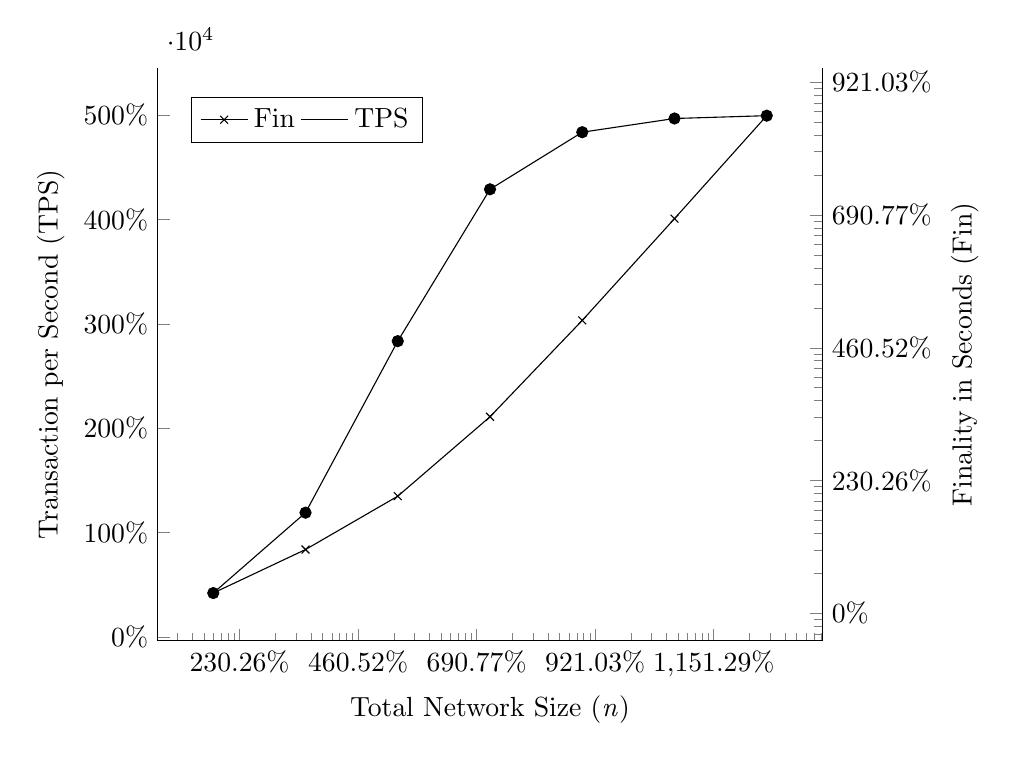
\begin{tikzpicture}
      \pgfplotsset{
          scale only axis,
      }
    
      \begin{axis}[
        xmode=log,
        axis y line*=left,
        axis x line*=bottom,
        xlabel = Total Network Size (\textit{n}),
        ylabel= Transaction per Second (TPS),   
        scaled y ticks=true
      ]
        \addplot[mark=*]
          coordinates{
            (6,4225.35)	
            (36,11920.49)	
            (216,28346.26)	
            (1296, 42885.46)	
            (7776,48351.61)	
            (46656,49664.07)	
            (279936,49934.27)
            % more points
          }; \label{plot_1}
    
        \end{axis}
    
        \begin{axis}[
          xmode=log,
          ymode=log,
          axis y line*=right,
          axis x line*=bottom,
          axis x line=none,
          ylabel=Finality in Seconds (Fin),
          legend style={at={(0.05,0.95)}, anchor=north west, legend cell align=left},
        ]
    
        \addplot[mark=x]
          coordinates{
            (6,1.42)	
            (36,3.02)	
            (216,7.62)	
            (1296, 30.22)	
            (7776,160.82)	
            (46656,939.43)	
            (279936,5606.09)			
            % more points
          }; \label{plot_2}
        \addlegendimage{/pgfplots/refstyle=plot_1}\addlegendentry{Fin}
        \addlegendimage{/pgfplots/refstyle=plot_2}\addlegendentry{TPS}
        \end{axis}
    \end{tikzpicture}
    \caption{The network throughput and finality as the number of network members increases, assuming the network is under maximum possible load.}
    \label{fig:proj_small}
\end{figure}
\begin{figure}[h!]
    \centering
    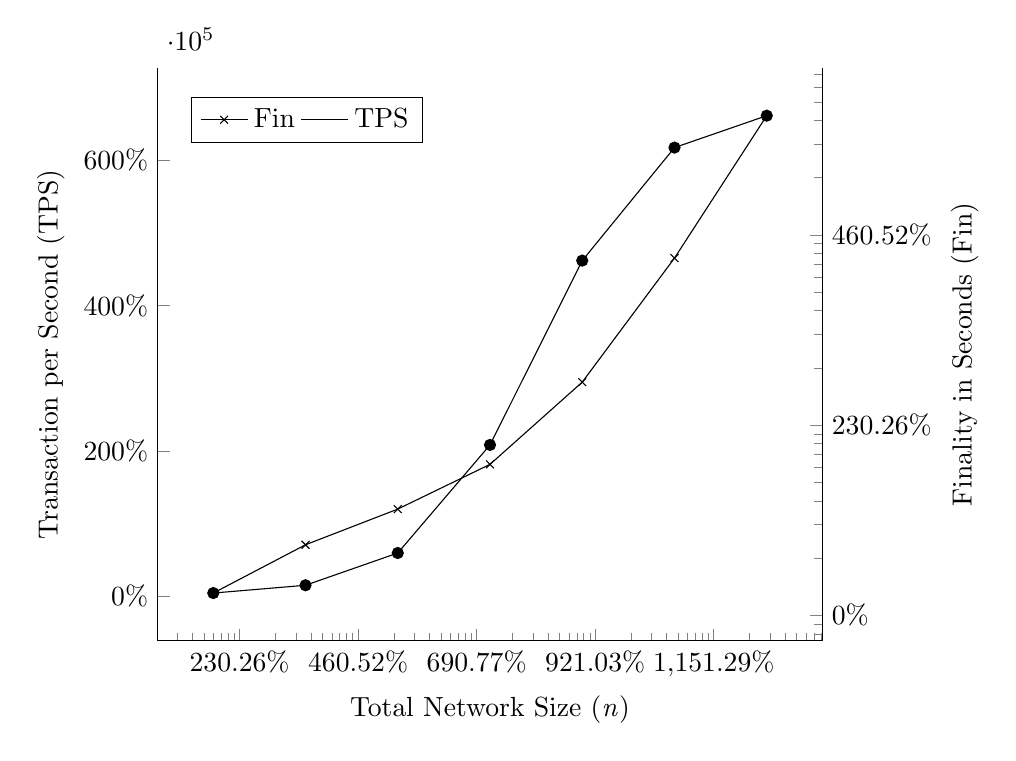
\begin{tikzpicture}
      \pgfplotsset{
          scale only axis,
      }
    
      \begin{axis}[
        xmode=log,
        axis y line*=left,
        axis x line*=bottom,
        xlabel = Total Network Size (\textit{n}),
        ylabel= Transaction per Second (TPS),   
        scaled y ticks=true
      ]
        \addplot[mark=*]
          coordinates{
            (6,4584.13)	
            (36,15298.09)	
            (216,59673.05)	
            (1296, 208362.67)	
            (7776,461963.52)	
            (46656,617451.49)	
            (279936,661354.75)
            % more points
          }; \label{plot_1}
    						
        \end{axis}
    
        \begin{axis}[
          xmode=log,
          ymode=log,
          axis y line*=right,
          axis x line*=bottom,
          axis x line=none,
          ylabel=Finality in Seconds (Fin),
          legend style={at={(0.05,0.95)}, anchor=north west, legend cell align=left},
        ]
    
        \addplot[mark=x]
          coordinates{
            (6,1.31)	
            (36,2.35)	
            (216,3.62)	
            (1296, 6.22)	
            (7776,16.83)	
            (46656,75.56)	
            (279936,423.28)			
            % more points
          }; \label{plot_2}
        \addlegendimage{/pgfplots/refstyle=plot_1}\addlegendentry{Fin}
        \addlegendimage{/pgfplots/refstyle=plot_2}\addlegendentry{TPS}
        \end{axis}
    \end{tikzpicture}
    \caption{The network throughput and finality as the number of network members increases, assuming the network is under maximum possible load.}
    \label{fig:proj_large}
\end{figure}


\begin{figure}[h!]
    \centering
    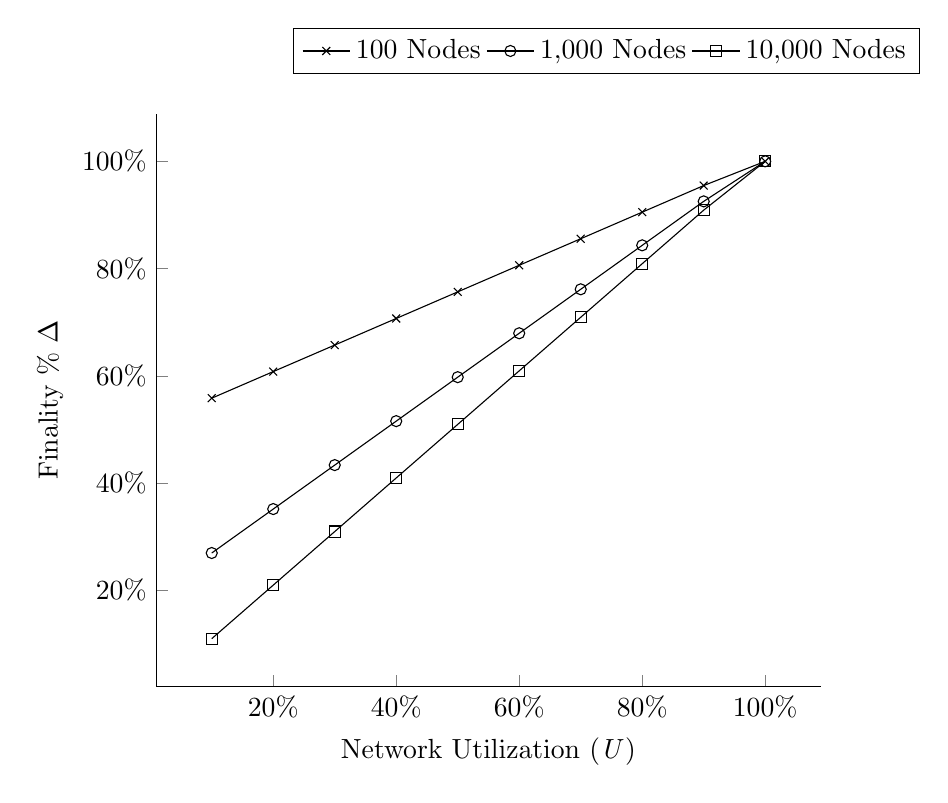
\begin{tikzpicture}
      \pgfplotsset{
          scale only axis,
          xticklabel={\pgfmathparse{\tick*100}\pgfmathprintnumber{\pgfmathresult}\%},
          yticklabel={\pgfmathparse{\tick*100}\pgfmathprintnumber{\pgfmathresult}\%},
          every axis legend/.append style={ at={(1.15,1.15)}, 
          legend columns = 0}
          % legend style={at={(0.5,0.5)},
      }
    
      \begin{axis}[
        % xmode=log,
        % ymode=log,
        axis y line*=left,
        axis x line*=bottom,
        xlabel = Network Utilization (\textit{U}),
        ylabel= Finality \(\%\) \(\Delta\),   
        scaled y ticks=true
      ]

        \addplot[mark=x,color=black] coordinates{
            (1, 1)
            (.9,.9548)
            (.8,.9052)
            (.7,.8556)
            (.6,.8061)
            (.5,.7565)
            (.4,.7069)
            (.3,.6573)
            (.2,.6078)
            (.1,.5582)
            % more points
          }; \label{plot_1_y1}
    
        \addplot[mark=o,color=black] coordinates{
            (1, 1)
            (.9,.9253)
            (.8,.8433)
            (.7,.7613)
            (.6,.6793)
            (.5,.5974)
            (.4,.5154)
            (.3,.4334)
            (.2,.3514)
            (.1,.2694)
            % more points
          }; \label{plot_1_y2}
          
        \addplot[mark=square,color=black] coordinates{
            (1, 1)
            (.9,.9089)
            (.8,.809)
            (.7,.7091)
            (.6,.6092)
            (.5,.5093)
            (.4,.4094)
            (.3,.3094)
            (.2,.2095)
            (.1,.1096)
            % more points
          }; \label{plot_1_y3}

%           100 %	1	1	1
% 90 %	0.9548	0.9253	0.9089
% 80 %	0.9052	0.8433	0.809
% 70 %	0.8556	0.7613	0.7091
% 60 %	0.8061	0.6793	0.6092
% 50%	0.7565	0.5974	0.5093
% 40 %	0.7069	0.5154	0.4094
% 30 %	0.6573	0.4334	0.3094
% 20 %	0.6078	0.3514	0.2095
% 10 %	0.5582	0.2694	0.1096
        
        \addlegendimage{/pgfplots/refstyle=plot_1_y1}\addlegendentry{100 Nodes}
        \addlegendimage{/pgfplots/refstyle=plot_1_y2}\addlegendentry{1,000 Nodes}
        \addlegendimage{/pgfplots/refstyle=plot_1_y3}\addlegendentry{10,000 Nodes}

        \end{axis}
    \end{tikzpicture}
    \caption{The percentage decrease in finality time as \textit{network utilization} decreases.}
    \label{fig:fin_change}
\end{figure}


\begin{figure}[h!]
    \centering
    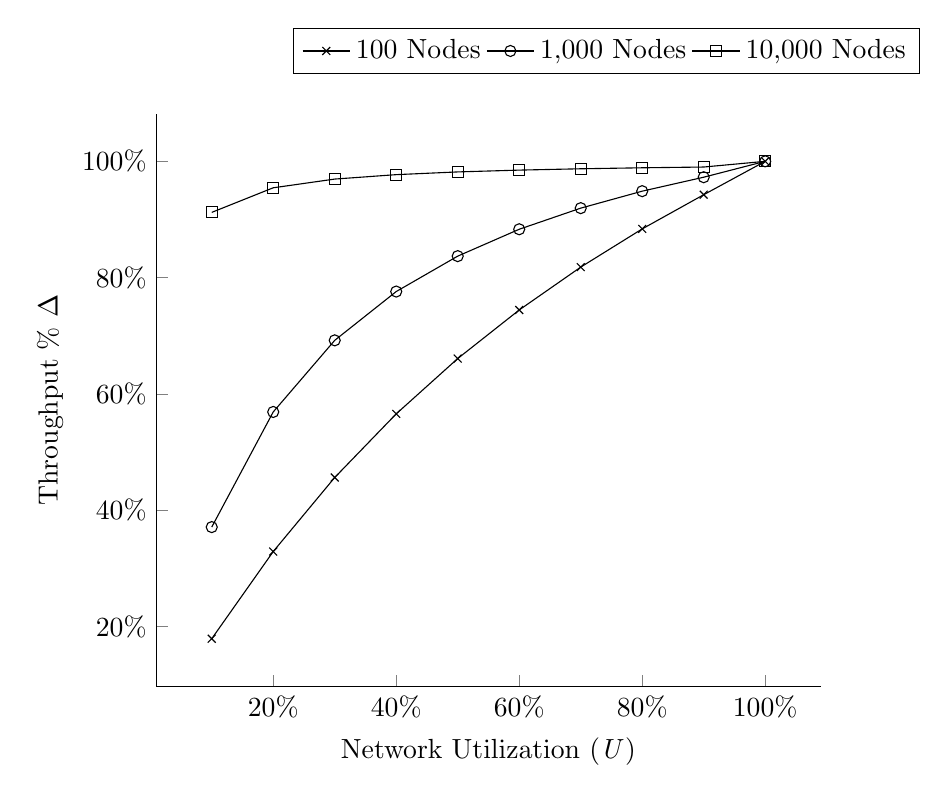
\begin{tikzpicture}
      \pgfplotsset{
          scale only axis,
          xticklabel={\pgfmathparse{\tick*100}\pgfmathprintnumber{\pgfmathresult}\%},
          yticklabel={\pgfmathparse{\tick*100}\pgfmathprintnumber{\pgfmathresult}\%},
          every axis legend/.append style={ at={(1.15,1.15)}, 
          legend columns = 0}
          % legend style={at={(0.5,0.5)},
      }
    
      \begin{axis}[
        % xmode=log,
        % ymode=log,
        axis y line*=left,
        axis x line*=bottom,
        xlabel = Network Utilization (\textit{U}),
        ylabel= Throughput \(\%\) \(\Delta\),   
        scaled y ticks=true
      ]

        \addplot[mark=x,color=black] coordinates{
            (1, 1)
            (.9,.9426)
            (.8,.8838)
            (.7,.8181)
            (.6,.7444)
            (.5,.6609)
            (.4,.5658)
            (.3,.4564)
            (.2,.3291)
            (.1,.1792)
            % more points
          }; \label{plot_1_y1}
    
        \addplot[mark=o,color=black] coordinates{
            (1, 1)
            (.9,.9727)
            (.8,.9487)
            (.7,.9195)
            (.6,.8832)
            (.5,.837)
            (.4,.7761)
            (.3,.6922)
            (.2,.5691)
            (.1,.3711)
            % more points
          }; \label{plot_1_y2}
          
        \addplot[mark=square,color=black] coordinates{
            (1, 1)
            (.9,.9902)
            (.8,.9889)
            (.7,.9872)
            (.6,.9849)
            (.5,.9818)
            (.4,.9771)
            (.3,.9695)
            (.2,.9545)
            (.1,.9122)
            % more points
          }; \label{plot_1_y3}

% 100 %	1	1	1
% 90 %	0.9426	0.9727	0.9902
% 80 %	0.8838	0.9487	0.9889
% 70 %	0.8181	0.9195	0.9872
% 60 %	0.7444	0.8832	0.9849
% 50%	0.6609	0.837	0.9818
% 40 %	0.5658	0.7761	0.9771
% 30 %	0.4564	0.6922	0.9695
% 20 %	0.3291	0.5691	0.9545
% 10 %	0.1792	0.3711	0.9122
        
        \addlegendimage{/pgfplots/refstyle=plot_1_y1}\addlegendentry{100 Nodes}
        \addlegendimage{/pgfplots/refstyle=plot_1_y2}\addlegendentry{1,000 Nodes}
        \addlegendimage{/pgfplots/refstyle=plot_1_y3}\addlegendentry{10,000 Nodes}

        \end{axis}
    \end{tikzpicture}
    \caption{The percentage decrease in finality time as \textit{network utilization} decreases.}
    \label{fig:tps_change}
\end{figure}


\begin{figure}[h!]
    \centering
    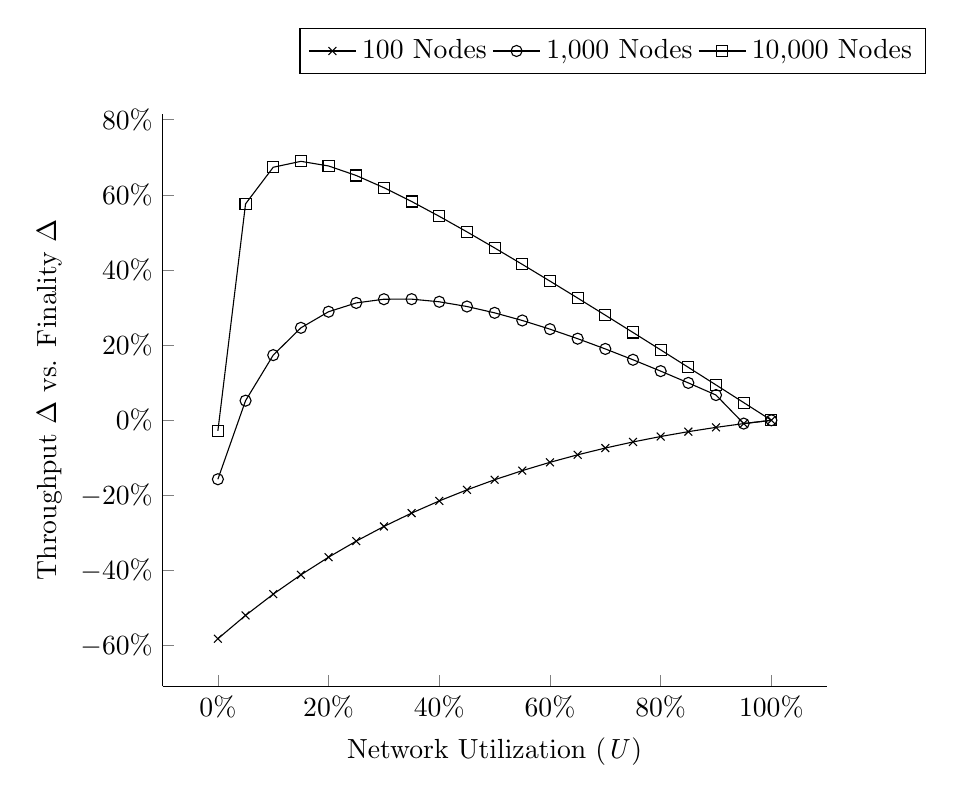
\begin{tikzpicture}
      \pgfplotsset{
          scale only axis,
          xticklabel={\pgfmathparse{\tick*100}\pgfmathprintnumber{\pgfmathresult}\%},
          yticklabel={\pgfmathparse{\tick*100}\pgfmathprintnumber{\pgfmathresult}\%},
          every axis legend/.append style={ at={(1.15,1.15)}, 
          legend columns = 0}
          % legend style={at={(0.5,0.5)},
      }
    
      \begin{axis}[
        % xmode=log,
        % ymode=log,
        axis y line*=left,
        axis x line*=bottom,
        xlabel = Network Utilization (\textit{U}),
        ylabel= Throughput \(\Delta\) vs. Finality \(\Delta\),   
        scaled y ticks=true
      ]

        \addplot[mark=x,color=black] coordinates{
            (1, 0)
            (.95,-0.00875085086638261)
            (.9,-0.0187989993125319)
            (.85,-0.0302313835961472)
            (.8,-0.043142887679075)
            (.75,-0.0576372701980755)
            (.7,-0.0738282268886817)
            (.65,-0.0918406093775239)
            (.6,-0.111811827868503)
            (.55,-0.133893470928493)
            (.5,-0.158253182612207)
            (.45,-0.185076845921641)
            (.4,-0.214571132554597)
            (.35,-0.246966492692794)
            (.3,-0.282520676053356)
            (.25,-0.321522897700105)
            (.2,-0.364298790694081)
            (.15,-0.411216324607017)
            (.1,-0.462692917036203)
            (.05,-0.519204028427371)
            (0,-0.58129361415549)
            % more points
          }; \label{plot_1_y1}
    
        \addplot[mark=o,color=black] coordinates{
            (1, 0)
            (.95,-0.00875085086638261)
            (.9,0.0671847318090388)
            (.85,0.0995370500255989)
            (.8,0.130894988501679)
            (.75,0.161099197548425)
            (.7,0.189954358332614)
            (.65,0.217218427009953)
            (.6,0.242587773750984)
            (.55,0.265676264596652)
            (.5,0.285985195910287)
            (.45,0.302859047758218)
            (.4,0.315418586808512)
            (.35,0.322456529299965)
            (.3,0.322268803136743)
            (.25,0.31236971536466)
            (.2,0.288985767560599)
            (.15,0.246097568383557)
            (.1,0.173476883918847)
            (.05,0.0522287880223851)
            (0,-0.156854896504616)	
            % more points
          }; \label{plot_1_y2}
          
        \addplot[mark=square,color=black] coordinates{
            (1, 0)
            (.95,0.0471276542363689)
            (.9,0.0940968333734938)
            (.85, 0.140880488190999)
            (.8,0.187445042266364)
            (.75,0.233748296740241)
            (.7,0.279736472626588)
            (.65,0.325339945982043)
            (.6,0.370466948376922)
            (.55,0.414994002319199)
            (.5,0.458750930637346)
            (.45,0.501496473543257)
            (.4,0.542876847340344)
            (.35,0.582351483992011)
            (.3,0.61905101794546)
            (.25,0.651482469380805)
            (.2,0.676847892643414)
            (.15,0.689219914258163)
            (.1,0.673468247744901)
            (0.05,0.576068249959748)
            (0,-0.0280081003964768)
            % more points
          }; \label{plot_1_y3}

% 	100 Nodes  (TPS)	1,000 Nodes (TPS)	10,000 Nodes (TPS)
% 100%	0	0	0
% 99%	-0.00165031375594715	0.00684956447079943	0.00943708890651074
% 98%	-0.00334992326651384	0.0136719962067303	0.018868570639354
% 97%	-0.00509945562212089	0.020466591092681	0.0282942767837751
% 96%	-0.00689954859475705	0.0272326204378547	0.0377140321122289
% 95%	-0.00875085086638261	0.0339693298941305	0.0471276542363689
% 94%	-0.0106540222632201	0.0406759383167853	0.0565349532374789
% 93%	-0.0126097339961068	0.0473516365639654	0.0659357312737873
% 92%	-0.0146186689070948	0.053995586231038	0.0753297821629385
% 91%	-0.0166815217224916	0.0606069183156491	0.0847168909377868
% 90%	-0.0187989993125319	0.0671847318090388	0.0940968333734938
% 89%	-0.0209718209578902	0.0737280922088006	0.103469375483743
% 88%	-0.0232007186232419	0.0802360299479392	0.112834272983696
% 87%	-0.0254864372380927	0.0867075387346703	0.1221912707171
% 86%	-0.027829734985105	0.0931415737969925	0.131540102044715
% 85%	-0.0302313835961472	0.0995370500255989	0.140880488190999
% 84%	-0.0326921686563201	0.105892840008188	0.150212137545661
% 83%	-0.0352128899162063	0.112207771947697	0.159534744916431
% 82%	-0.0377943616125981	0.118480627456378	0.168847990729
% 81%	-0.0404374127979855	0.124710139216991	0.178151540169741
% 80%	-0.043142887679075	0.130894988501679	0.187445042266364
% 79%	-0.0459116459646319	0.137033802538329	0.196728128901203
% 78%	-0.0487445632229522	0.143125151713345	0.206000413751314
% 77%	-0.0516425312492659	0.149167546598887	0.215261491148955
% 76%	-0.0546064584434062	0.155159434791552	0.224510934855392
% 75%	-0.0576372701980755	0.161099197548425	0.233748296740241
% 74%	-0.0607359092980535	0.16698514620517	0.242973105357741
% 73%	-0.0639033363307175	0.172815518359506	0.252184864410451
% 72%	-0.0671405301082428	0.178588473801943	0.261383051089853
% 71%	-0.0704484881018747	0.184302090174034	0.270567114282188
% 70%	-0.0738282268886817	0.189954358332614	0.279736472626588
% 69%	-0.0772807826112031	0.195543177396536	0.288890512411124
% 68%	-0.0808072114504299	0.201066349450237	0.298028585290751
% 67%	-0.0844085901125768	0.206521573876075	0.30715000580932
% 66%	-0.08808601633011	0.211906441284722	0.316254048705741
% 65%	-0.0918406093775239	0.217218427009953	0.325339945982043
% 64%	-0.0956735106023761	0.22245488413093	0.334406883708403
% 63%	-0.0995858839721068	0.227613035981431	0.343453998537203
% 62%	-0.103578916637198	0.232689968101487	0.352480373894715
% 61%	-0.107653819511241	0.23768261958238	0.361485035815107
% 60%	-0.111811827868503	0.242587773750984	0.370466948376922
% 59%	-0.116054201959627	0.247402048133861	0.379425008697098
% 58%	-0.120382227646092	0.252121883635285	0.388358041431626
% 57%	-0.124797217054114	0.256743532856419	0.397264792725189
% 56%	-0.129300509248689	0.261263047475068	0.406143923544275
% 55%	-0.133893470928493	0.265676264596652	0.414994002319199
% 54%	-0.138577497142414	0.26997879197721	0.423813496809984
% 53%	-0.143354012028482	0.274165992008181	0.432600765098886
% 52%	-0.148224469576048	0.278232964340179	0.44135404559816
% 51%	-0.153190354412039	0.282174527008895	0.450071445945142
% 50%	-0.158253182612207	0.285985195910287	0.458750930637346
% 49%	-0.163414502538282	0.289659162454145	0.467390307237591
% 48%	-0.168675895702019	0.293190269204561	0.475987210952416
% 47%	-0.174038977657137	0.296571983292516	0.484539087355514
% 46%	-0.179505398920214	0.29979736735919	0.493043172990538
% 45%	-0.185076845921641	0.302859047758218	0.501496473543257
% 44%	-0.190755041987778	0.305749179710422	0.509895739220138
% 43%	-0.196541748355527	0.308459409064707	0.518237436907147
% 42%	-0.202438765220558	0.310980830273137	0.526517718606584
% 41%	-0.208447932820523	0.313303940135568	0.534732385558236
% 40%	-0.214571132554597	0.315418586808512	0.542876847340344
% 39%	-0.220810288140806	0.317313913502764	0.550946075111317
% 38%	-0.227167366812617	0.318978296212942	0.558934547988946
% 37%	-0.233644380556359	0.320399274727637	0.566836191362599
% 36%	-0.240243387391116	0.321563476058732	0.574644305686068
% 35%	-0.246966492692794	0.322456529299965	0.582351483992011
% 34%	-0.253815850564154	0.323062970774183	0.589949515987391
% 33%	-0.260793665252686	0.323366138151968	0.597429276112036
% 32%	-0.267902192618279	0.323348052016039	0.604780592342059
% 31%	-0.275143741652748	0.322989283099795	0.611992091759971
% 30%	-0.282520676053356	0.322268803136743	0.61905101794546
% 29%	-0.290035415852594	0.321163816910848	0.625943013999696
% 28%	-0.297690439106577	0.319649572684094	0.632651863413209
% 27%	-0.305488283644525	0.317699147682258	0.639159178901855
% 26%	-0.313431548881925	0.315283204724551	0.645444026599893
% 25%	-0.321522897700105	0.31236971536466	0.651482469380805
% 24%	-0.329765058395059	0.308923644040806	0.657247008246536
% 23%	-0.338160826698525	0.304906586674421	0.662705894216418
% 22%	-0.346713067874472	0.300276355864411	0.667822274283021
% 21%	-0.355424718894278	0.294986503237705	0.672553122797663
% 20%	-0.364298790694081	0.288985767560599	0.676847892643414
% 19%	-0.373338370517947	0.282217434791059	0.680646796554293
% 18%	-0.382546624350676	0.274618593231741	0.683878594596515
% 17%	-0.391926799444289	0.266119263159504	0.686457713938461
% 16%	-0.40148222694241	0.2566413755391	0.688280453366783
% 15%	-0.411216324607017	0.246097568383557	0.689219914258163
% 14%	-0.421132599652237	0.234389761609904	0.689119129925581
% 13%	-0.431234651690136	0.221407461328243	0.687781599247454
% 12%	-0.441526175793677	0.20702573167703	0.684958003600565
% 11%	-0.452010965682347	0.191102755593143	0.680327182460175
% 10%	-0.462692917036203	0.173476883918847	0.673468247744901
% 9%	-0.473576030944429	0.153963043092706	0.663818616294178
% 8%	-0.48466441749481	0.132348332653256	0.650608901715372
% 7%	-0.495962299510891	0.108386591050549	0.632758272932124
% 6%	-0.507474016443957	0.081791636236959	0.60869912111628
% 5%	-0.519204028427371	0.0522287880223851	0.576068249959748
% 4%	-0.531156920501221	0.0193041400804878	0.531128814459303
% 3%	-0.543337407015695	-0.0174491475540527	0.467602553340845
% 2%	-0.555750336222049	-0.0585885477774608	0.374066687520415
% 1%	-0.568400695060574	-0.104785282879006	0.227326975834317
% 0%	-0.58129361415549	-0.156854896504616	-0.0280081003964768
        
        \addlegendimage{/pgfplots/refstyle=plot_1_y1}\addlegendentry{100 Nodes}
        \addlegendimage{/pgfplots/refstyle=plot_1_y2}\addlegendentry{1,000 Nodes}
        \addlegendimage{/pgfplots/refstyle=plot_1_y3}\addlegendentry{10,000 Nodes}

        \end{axis}
    \end{tikzpicture}
    \caption{The percentage change in throughput versus the change in finality as \textit{network utilization} is reduced.}
    \label{fig:comp_change}
\end{figure}
